\chapter{Desarrollo experimental}
	
	Este trabajo busca realizar una investigación cuasi-experimental para reportar el comportamiento  del destilador solar propuesto de acuerdo a la influencia de las variables independientes descritas en la~\cref{table:variables-independientes-desarrollo-experimental}.
	
	\begin{longtblr}[
		caption = {Variables del desarrollo experimental},
		label = {table:variables-independientes-desarrollo-experimental},
		note{*} = {Se puede ejercer control directo sobre esta variable.}
	]{
		colspec = {X[l] c c X[2, l]},
		hlines,
		vlines,
		row{odd} = {bg=tablerowblue},
		row{1} = {
			bg = tabletitleblue,
			fg=white,
			font = \bfseries,
			halign=c
		},
		rowhead = 1,
		rows={m}
	}
		Variable & Clasificación & Tipo de dato & Influencia en el modelo\\
		Temperatura de entrada del agua\TblrNote{*}
			& Independiente
			& Cuantitativa
			& Establece la temperatura inicial del modelo térmico para la ebullición del agua\\
		Presión atmosférica
			& Independiente
			& Cuantitativa
			& Modifica la temperatura a la cual sucede el cambio de fase del agua\\
		Temperatura ambiente
			& Independiente
			& Cuantitativa
			& Influye en las pérdidas de calor que tendrá el sistema\\
		Clima (nubosidad)
			& Independiente
			& Cualitativa
			& Punto de comparación rápido para ver la influencia de la nubosidad sobre el desempeño\\
		Velocidad de viento
			& Independiente
			& Cuantitativa
			& Se asocia directamente a las pérdidas de calor por convección\\
		Hola del día
			& Independiente
			& Cuantitativa
			& Determina la posición angular del Sol y se relaciona con la irradiación solar\\
		Irradiación solar promedio
			& Independiente
			& Cuantitativa
			& Determina la potencia solar recibida en nuestro modelo de transferencia de calor\\
		Temperatura de salida del agua
			& Dependiente
			& Cuantitativa
			& Asociada al cambio de fase del agua\\
		Temperatura del recibidor solar
			& Dependiente
			& Cuantitativa
			& Influye en los modelos térmicos para la destilación del agua\\
		Caudal de agua\TblrNote{*} 
			& Dependiente
			& Cuantitativa
			& Influye en los modelos térmicos y la tasa de desalinización\\
		Propiedades físico-químicas del agua
			& Dependiente
			& Cuantitativa
			& Indica la calidad del agua
	\end{longtblr}
	
	\section{Grupos de estudio}
		
		Con base en las variables observadas en la~\cref{table:variables-independientes-desarrollo-experimental} se distinguieron los grupos de control descritos en las sub-secciones siguientes.
		
		\subsection{Agua}
			
			Las muestras de agua se seleccionaron guiándose en la~\cref{table:clasificacion-agua-tds}. Para ello, la obtención de agua de mar se simula con sales marinas para acuario y se proponen 3 grupos de estudio descritos en la~\cref{table:grupo-control-agua} para evaluar los casos límite y promedio de la salinidad del agua de mar.
			
			\begin{longtblr}[
				caption = {Grupo de estudio del agua de mar},
				label = {table:grupo-control-agua}
			]{
				colspec = {X[c] X[2, c]},
				hlines,
				vlines,
				width = 0.5\linewidth,
				rowhead = 1,
				row{odd} = {bg=tablerowblue},
				row{1} = {
					bg = tabletitleblue,
					fg=white,
					font = \bfseries,
					halign=c
				},
				rows={m}
			}
				Muestra & Salinidad (\unit{\mg\per\litre})\\
				1 & \num{30000}\\
				2 & \num{35000}\\
				3 & \num{40000}
			\end{longtblr}
		
		\subsection{Lugar físico de experimentación}\label{sec:ch6-lugar-fisico}
			
			Debido al alcance del proyecto, se acotó el lugar físico de experimentación a la Unidad Profesional Interdisciplinaria en Ingeniería y Tecnologías Avanzadas ubicada en la Ciudad de México.
			
			\begin{longtblr}[
				caption = {Coordenadas geográficas},
				label = {table:grupo-control-fisico}
			]{
				colspec = {X[c] *{3}{c}},
				hlines,
				vlines,
				width = 0.8\linewidth,
				rowhead = 1,
				row{odd} = {bg=tablerowblue},
				row{1} = {
					bg = tabletitleblue,
					fg=white,
					font = \bfseries,
					halign=c
				},
				rows={m}
			}
				Zona & Longitud & Latitud & Altitud\\
				Ciudad de México, México
					& \ang{-99;07;32}
					& \ang{19;30;38}
					& \qty{2241}{\m}
			\end{longtblr}
			
			\subsubsection{Variables climáticas sobre la región a investigar}
				
				Debido a la naturaleza de nuestra fuente de energía y que su operación no transcurren dentro de un ambiente controlado se deben evaluar las condiciones climáticas del lugar que impactan en mayor medida el sistema propuesto.
				
				\begin{longtblr}[
					caption = {Variables climáticas consideradas importantes para la investigación},
					label = {table:variables-climaticas},
					note{?} = {Estas variables fueron estudiadas para saber si se debían considerar en los modelos a desarrollar, sin embargo, tras un segundo análisis después del estudio se decició excluirlas del modelo }
				]{
					colspec = {X[c] X[3, l] c},
					hlines,
					vlines,
					width = \linewidth,
					row{odd} = {bg=tablerowblue},
					rowhead = 1,
					row{1} = {
						bg = tabletitleblue,
						fg=white,
						font = \bfseries,
						halign=c
					},
					rows={m}
				}
					Variable & Descripción & Unidades\\
					Presión superficial
						& Presión promedio en la superficie del lugar
						& \unit{\kilo\pascal}\\
					Velocidad de viento
						& Velocidad de viento promedio a 2 metros sobre la superficie del lugar
						& \unit{\m\per\s}\\
					Humedad específica
						& Razón promedio de la masa de vapor de agua por unidad de aire a 2 metros sobre la superficie del lugar
						& \unit{\gram\per\kg}\\
					\acrfull{roc} sobre cielo despejado
						& Total de irradiación solar incidida (directa más difusa) sobre la tierra en un plano horizontal sobre la superficie de la tierra a condiciones de cielo despejado.
						& \unit{\watt\hour\per\m\tothe{2}}\\
					\acrlong{roc}
						& Total de irradiación solar incidida (directa más difusa) sobre la tierra en un plano horizontal sobre la superficie de la tierra a todas las condiciones.
						& \unit{\watt\hour\per\m\tothe{2}}\\
					Nubosidad
						& Porcentaje promedio de cantidad de nubes en el cielo sobre un lapso determinado
						& \unit{\watt\hour\per\m\tothe{2}}\\
					Irradiancia UVA\TblrNote{?}
						& Radiación UVA (\qtyrange{315}{400}{\nm}) total incidida a todas las condiciones climáticas del día
						& \unit{\watt\per\m\tothe{2}}\\
					Irradiancia UVB\TblrNote{?}
						& Radiación UVB (\qtyrange{280}{315}{\nm}) total incidida a todas las condiciones climáticas del día
						& \unit{\watt\per\m\tothe{2}}	
				\end{longtblr}

	\section{Descripción de los problemas asociados a la destilación solar}
		
		Gracias a una entrevista informal con el Dr. Sergio Isai Palomino Resendiz acerca del modelo propuesto en \cite{palomino-resendiz_design_2018}, se identificó que la humedad suele condensarse sobre el vidrio o cristal afectando así la transmisividad y por ende el calor efectivo que llega al agua. Además, debido a la naturaleza intermitente de la energía solar, el proceso de desalinización suele presentar caídas grandes de producción en presencia de una nube.
		
		Por ello, este diseño se encaminó a mitigar en lo posible los problemas identificados proponiendo un método de almacenamiento de energía térmica y transferencia indirecta de calor.
		
	\section{Configuración experimental}
		
		Para definir los criterios de operación sobre los cuales se espera que opere en pruebas el sistema, se realizó un análisis de datos de las variables climáticas propuestas. Los datos utilizados fueron obtenidos de \textit{NASA Langley Research Center (LaRC) POWER Project} financiado por el Programa de Ciencias de la Tierra/Ciencias Aplicadas de la NASA usando el código mostrado en el \cref{ch:solar-irradiation-code}.
		
		De dicho código se obtuvieron gráficas de área que nos representaban el comportamiento reportado por \textit{The Power LaRC} en intervalos de cada hora.
	
		\subsection{Radiación solar de onda corta}
			
			En la~\cref{fig:SFC_SW_DWN} observamos que de marzo a septiembre tenemos los niveles más altos de \acrlong{roc} y esta radiación se encuentra dentro de un rango de \qtyrange{5}{8}{\kWh\per\m\tothe{2}\day}.
			
			De las~\cref{fig:ALLSKY_SFC_SW_DWN_3d_mean_2020,fig:ALLSKY_SFC_SW_DWN_3d_mean_2021} se observa que la irradiancia se de \acrshort{roc} de interés varía entre los \qtyrange{500}{900}{\watt\per\m\tothe{2}} y se aprecia que en mayor proporción se encuentra entre \qtyrange{600}{700}{\watt\per\m\tothe{2}} por lo que para los cálculos de operación se decide usar \qty{650}{\watt\per\m\tothe{2}} como valor de irradiancia.
	
			\begin{figure}[H]
				\centering
				\begin{subfigure}[t]{0.45\linewidth}
					\centering
					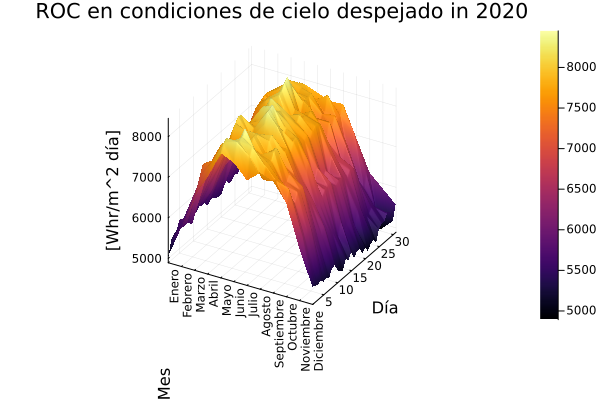
\includegraphics[
						width=\linewidth,
						height = 60mm,
						keepaspectratio
					]{Resultados/DataAnalysis/CLRSKY_SFC_SW_DWN_surface_2020_3d.png}
					\caption{Irradiación de onda corta total recibida por día en condiciones de cielo despejado durante el 2020 sobre el lugar seleccionado}
					\label{fig:CLRSKY_SFC_SW_DWN_surface_2020_3d}
				\end{subfigure}
				\hfill
				\begin{subfigure}[t]{0.45\linewidth}
					\centering
					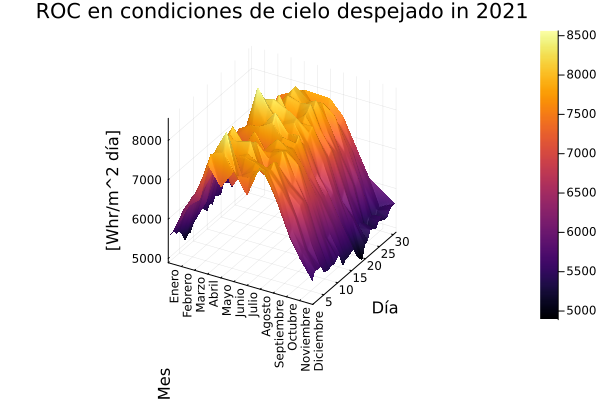
\includegraphics[
						width=\linewidth,
						height = 60mm,
						keepaspectratio
					]{Resultados/DataAnalysis/CLRSKY_SFC_SW_DWN_surface_2021_3d.png}
					\caption{Irradiación de onda corta total recibida por día en condiciones de cielo despejado durante el 2021 sobre el lugar seleccionado}
					\label{fig:CLRSKY_SFC_SW_DWN_surface_2021_3d}
				\end{subfigure}
			\end{figure}
			
			\begin{figure}[H]\ContinuedFloat
				\begin{subfigure}[t]{0.45\linewidth}
					\centering
					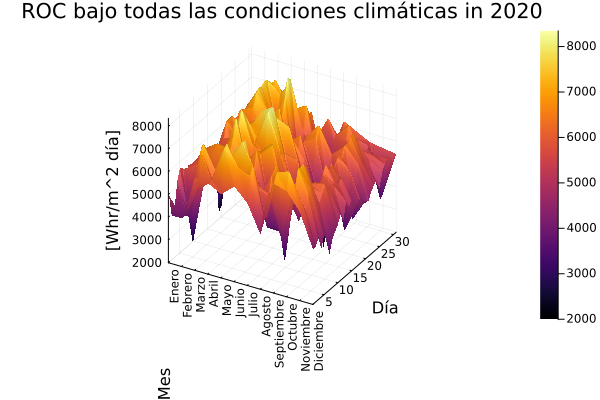
\includegraphics[
						width=\linewidth,
						height = 60mm,
						keepaspectratio
					]{Resultados/DataAnalysis/ALLSKY_SFC_SW_DWN_surface_2020_3d.png}
					\caption{Irradiación de onda corta total recibida por día bajo todas las condiciones climáticas durante el 2020 sobre el lugar seleccionado}
					\label{fig:ALLSKY_SFC_SW_DWN_surface_2020_3d}
				\end{subfigure}
				\hfill
				\begin{subfigure}[t]{0.45\linewidth}
					\centering
					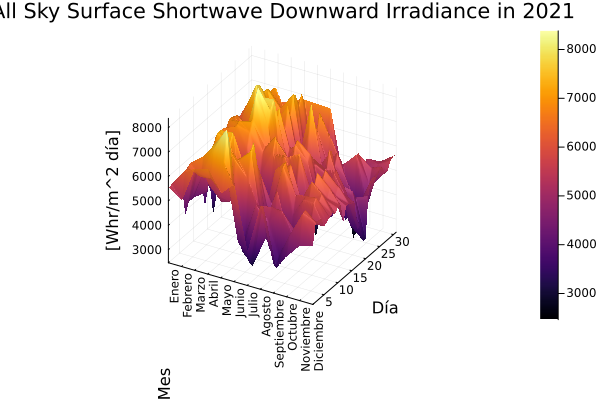
\includegraphics[
						width=\linewidth,
						height = 60mm,
						keepaspectratio
					]{Resultados/DataAnalysis/ALLSKY_SFC_SW_DWN_surface_2021_3d.png}
					\caption{Irradiación de onda corta total recibida por día bajo todas las condiciones climáticas durante el 2021 sobre el lugar seleccionado}
					\label{fig:ALLSKY_SFC_SW_DWN_surface_2021_3d}
				\end{subfigure}
			\end{figure}
			
			\begin{figure}[H]\ContinuedFloat
				\begin{subfigure}[t]{0.45\linewidth}
					\centering
					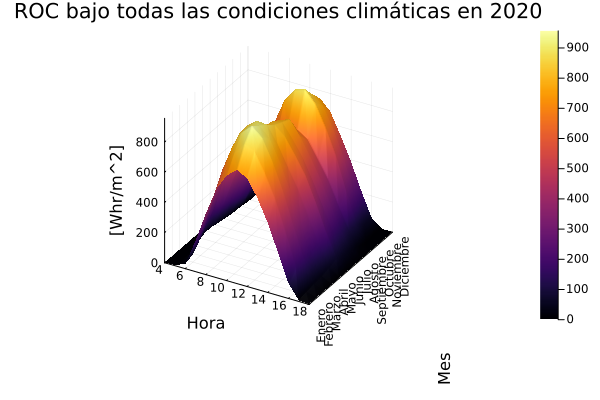
\includegraphics[
						width=\linewidth,
						height = 60mm,
						keepaspectratio
					]{Resultados/DataAnalysis/ALLSKY_SFC_SW_DWN_3d_mean_2020.png}
					\caption{Irradiación de onda corta promedio recibida por hora bajo todas las condiciones climáticas durante el 2020 sobre el lugar seleccionado}
					\label{fig:ALLSKY_SFC_SW_DWN_3d_mean_2020}
				\end{subfigure}
				\hfill
				\begin{subfigure}[t]{0.45\linewidth}
					\centering
					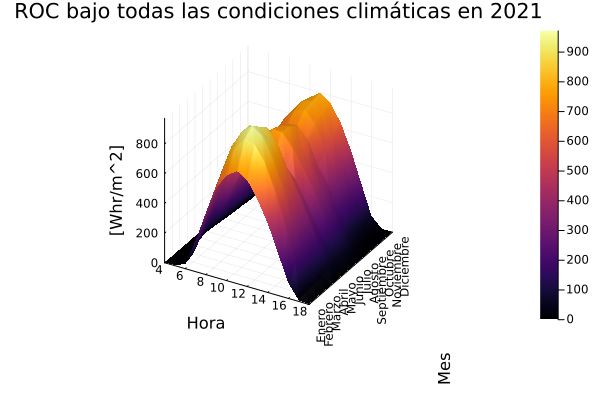
\includegraphics[
						width=\linewidth,
						height = 60mm,
						keepaspectratio
					]{Resultados/DataAnalysis/ALLSKY_SFC_SW_DWN_3d_mean_2021.png}
					\caption{Irradiación de onda corta promedio recibida por hora bajo todas las condiciones climáticas durante el 2021 sobre el lugar seleccionado}
					\label{fig:ALLSKY_SFC_SW_DWN_3d_mean_2021}
				\end{subfigure}
				\caption{Irradiación de onda corta recibida en el lugar físico de experimentación durante 2020 y 2021}
				\label{fig:SFC_SW_DWN}
			\end{figure}

		\subsection{Temperatura}
			
			Debido a que no se pudo obtener una base de datos que proporcionara la temperatura en intervalos de una hora, se decidió usar el resumen presentado por WeatherSpark, el cual se puede observar en la~\cref{fig:Temperatura-CDMX}.
			
			De la revisión de la~\cref{fig:Temperatura-CDMX} se observa que la temperatura mínima durante los meses de mayor radiación solar se tiene una temperatura mínima de \qty{13}{\degreeCelsius} y se define que la temperatura inicial del agua de entrada sería cercana a los \qty{15.5}{\degreeCelsius}. Para condiciones de operación en horas más avanzadas, el agua de entrada se encontraría entre los \qtyrange{18}{24}{\degreeCelsius}.
			
			\begin{figure}[H]
				\centering
				\begin{subfigure}[t]{\linewidth}
					\centering
					\includegraphics[
						width=\linewidth,
						height=70mm,
						keepaspectratio
					]{Resultados/DataAnalysis/Temperatura-promedio-por-hora-en-Ciudad-de-México.png}
					\\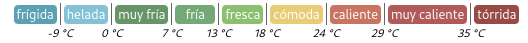
\includegraphics[
						width=0.8\linewidth,
						keepaspectratio
					]{Resultados/DataAnalysis/WeatherSpark-Temperatura-Leyenda.png}
					\caption{Temperatura promedio por hora en Ciudad de México}
					\label{fig:Temperatura-promedio-por-hora-en-Ciudad-de-México}
				\end{subfigure}
			\end{figure}
			\begin{figure}[H]\ContinuedFloat
				\begin{subfigure}[t]{\linewidth}
					\centering
					\includegraphics[
						width=\linewidth,
						height=70mm,
						keepaspectratio
					]{Resultados/DataAnalysis/Temperatura-por-hora-en-2022-Ciudad-de-México.png}\\
					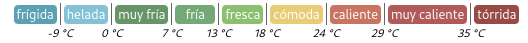
\includegraphics[
						width=0.8\linewidth,
						keepaspectratio
					]{Resultados/DataAnalysis/WeatherSpark-Temperatura-Leyenda.png}
					\caption{Temperatura por hora del 2022 en la Ciudad de México}
					\label{fig:Temperatura-por-hora-en-2022-Ciudad-de-México}
				\end{subfigure}
				\caption{Mapas de temperaturas de la Ciudad de México}
				\floatfoot{Los gráficos fueron obtenidos de \href{https://es.weatherspark.com/y/5674/Clima-promedio-en-Ciudad-de-México-México-durante-todo-el-año}{\textcopyright WeatherSpark.com}}
				\label{fig:Temperatura-CDMX}
			\end{figure}
		
		\subsection{Presión atmosférica}
			
			En la~\cref{fig:PS_3d_mean} se observa que la presión superficial varía muy poco, debido a ello sólo se tomará el valor redondeado de \qty{74.80}{\kilo\pascal} para cálculos posteriores.
			
			\begin{figure}[H]
				\centering
				\begin{subfigure}[t]{0.45\linewidth}
					\centering
					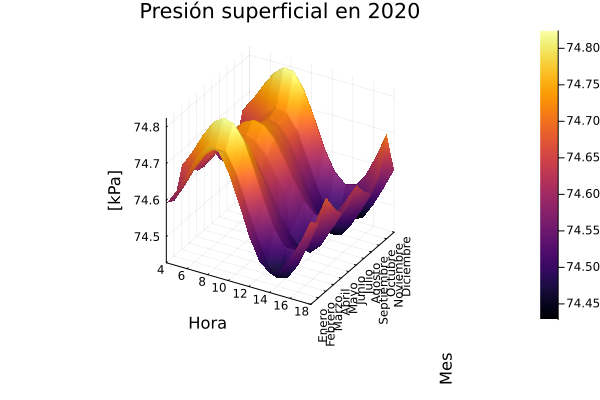
\includegraphics[
						width=\linewidth,
						height = 60mm,
						keepaspectratio
					]{Resultados/DataAnalysis/PS_3d_mean_2020.png}
					\caption{Presión promedio por hora del viento durante 2020 sobre el lugar seleccionado}
					\label{fig:PS_3d_mean_2020}
				\end{subfigure}
				\hfill
				\begin{subfigure}[t]{0.45\linewidth}
					\centering
					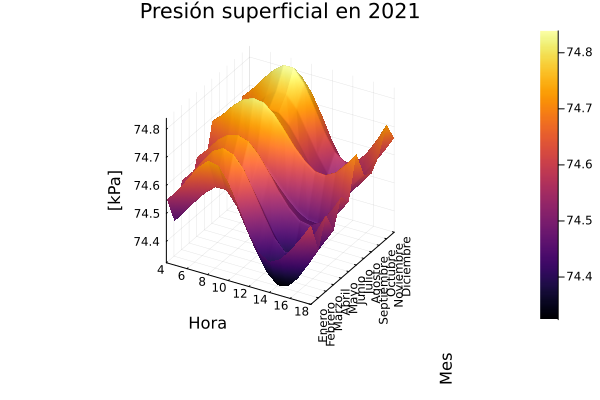
\includegraphics[
						width=\linewidth,
						height = 60mm,
						keepaspectratio
					]{Resultados/DataAnalysis/PS_3d_mean_2021.png}
					\caption{Presión promedio por hora del viento durante 2021 sobre el lugar seleccionado}
					\label{fig:PS_3d_mean_2021}
				\end{subfigure}
				\caption{Presión promedio en el lugar físico de experimentación durante 2020 y 2021}
				\label{fig:PS_3d_mean}
			\end{figure}
			
		\subsection{Magnitud del perfil de velocidad del viento}
		
			Debido a las pérdidas térmicas esperadas por convección forzada se estudió este criterio, sin embargo, como se observa en la~\cref{fig:WS2M_3d_mean} no se distingue visiblemente un patrón en el comportamiento. Se decidió usar un valor promedio de \qty{1.5}{\m\per\s}.
			
			\begin{figure}[H]
				\centering
				\begin{subfigure}[t]{0.45\linewidth}
					\centering
					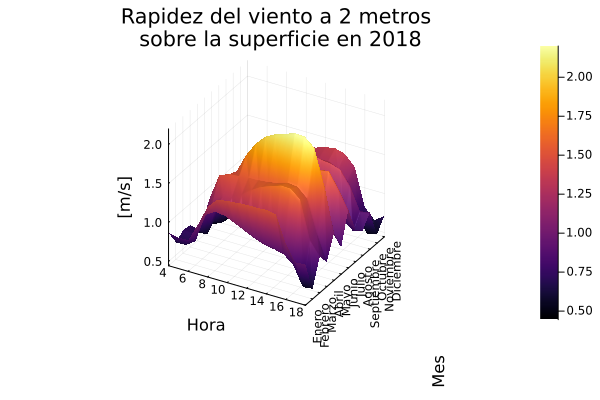
\includegraphics[
						width=\linewidth,
						height = 60mm,
						keepaspectratio
					]{Resultados/DataAnalysis/WS2M_3d_mean_2018.png}
					\caption{Rapidez promedio por hora del viento durante 2018 sobre el lugar seleccionado}
					\label{fig:WS2M_3d_mean_2018}
				\end{subfigure}
				\hfill
				\begin{subfigure}[t]{0.45\linewidth}
					\centering
					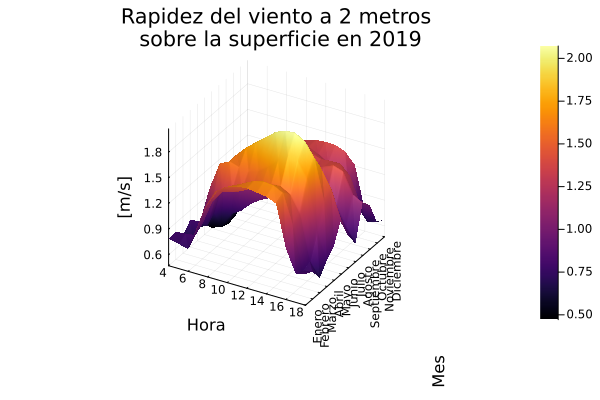
\includegraphics[
						width=\linewidth,
						height = 60mm,
						keepaspectratio
					]{Resultados/DataAnalysis/WS2M_3d_mean_2019.png}
					\caption{Rapidez promedio por hora del viento durante 2019 sobre el lugar seleccionado}
					\label{fig:WS2M_3d_mean_2019}
				\end{subfigure}
			\end{figure}
			
			\begin{figure}[H]\ContinuedFloat
				\begin{subfigure}[t]{0.45\linewidth}
					\centering
					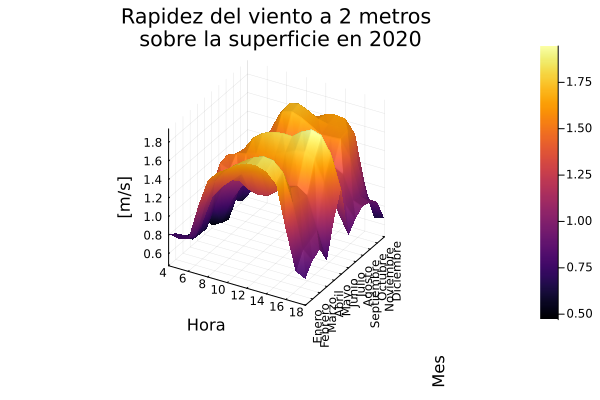
\includegraphics[
						width=\linewidth,
						height = 60mm,
						keepaspectratio
					]{Resultados/DataAnalysis/WS2M_3d_mean_2020.png}
					\caption{Rapidez promedio por hora del viento durante 2020 sobre el lugar seleccionado}
					\label{fig:WS2M_3d_mean_2020}
				\end{subfigure}
				\hfill
				\begin{subfigure}[t]{0.45\linewidth}
					\centering
					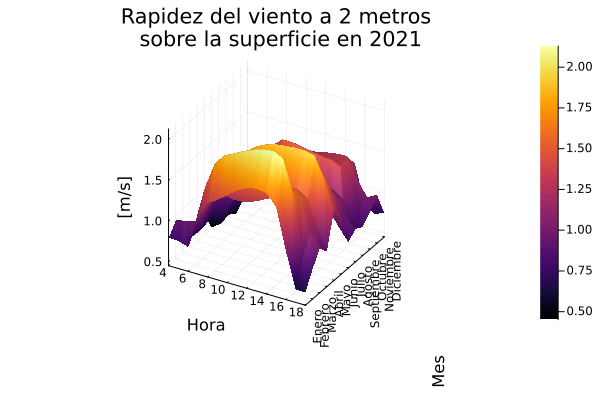
\includegraphics[
						width=\linewidth,
						height = 60mm,
						keepaspectratio
					]{Resultados/DataAnalysis/WS2M_3d_mean_2021.png}
					\caption{Rapidez promedio del viento durante 2021 sobre el lugar seleccionado}
					\label{fig:WS2M_3d_mean_2021}
				\end{subfigure}
				\caption{Rapidez promedio por hora del viento sobre el lugar seleccionado}
				\label{fig:WS2M_3d_mean}
			\end{figure}
	
		\subsection{Definición de valores esperados de la configuración experimental}
			
			Usando los límites de operación encontrados del análisis de datos se calcula mediante \eqref{equ:interpolación-lineal-simple} y los datos de los~\cref{ch:seawater-properties,ch:agua-saturada-propiedades} la temperatura de ebullición del agua de mar en el sitio de experimentación y a la cual se le agrega un \percent{2} de tolerancia.
			
			\begin{equation}\label{equ:interpolación-lineal-simple}
				y = y_{0} + \dfrac{y_{1}-y_{0}}{x_{1}-x_{0}} \times (x-x_{0})
			\end{equation}
			
			\begin{longtblr}[
				caption = {Datos a interpolar para definir los parámetros de salida del agua},
				label = {table:interpolación-agua-salida},
			]{
				colspec = {*{3}{X}},
				hlines,
				vlines,
				row{odd} = {bg=tablerowblue},
				row{1} = {
					bg = tabletitleblue,
					fg=white,
					font = \bfseries
				},
				width=0.75\linewidth,
				rowhead = 1,
				rows={
					valign = m,
					halign = c,
					mode = math
				}
			}
				~ & y & x\\
				0 & \qty{90}{\degreeCelsius} & \qty{70.14}{\kilo\pascal}\\
				1 & \qty{95}{\degreeCelsius} & \qty{80.55}{\kilo\pascal}\\
				\text{T}_{\text{salida}} & ~ & \qty{74.80}{\kilo\pascal}
			\end{longtblr}
			
			\begin{align*}
				\text{T}_{\text{ebullición agua dulce}} &= \qty{90}{\degreeCelsius} + \dfrac{\qty{95}{\degreeCelsius} - \qty{90}{\degreeCelsius}}{\qty{80.55}{\kilo\pascal}-\qty{70.14}{\kilo\pascal}} \times (\qty{74.80}{\kilo\pascal} - \qty{70.14}{\kilo\pascal})\\
				\text{T}_{\text{salida}} &= (\text{T}_{\text{ebullición agua dulce}} + \qty{0.601}{\degreeCelsius}) + \text{Tolerancia}\\
				\text{T}_{\text{salida}} &= (\qty{92.238}{\degreeCelsius} + \qty{0.601}{\degreeCelsius}) \times (1.02)\\
				\text{T}_{\text{salida}} &\approx \qty{94.70}{\degreeCelsius}
			\end{align*}
			
			Y considerando una temperatura de entrada del agua igual al inicio de sus operaciones de \qty{15.5}{\degreeCelsius} tenemos calculamos mediante \eqref{equ:potencia-necesaria-agua} el flujo de calor necesario por unidad de flujo másico que se necesita para lograr la ebullición del agua y el cambio de fase.
			
			\begin{equation}\label{equ:potencia-necesaria-agua}
				\dfrac{\dot{Q}}{\dot{m}} = \left(\gls{cs}_{\text{agua}} \Delta T + \gls{hl}\right)
			\end{equation}
			
			Para conocer $\gls{cs}_{\text{agua}}$ de la \cref{table:Calor-específico-agua} se usa \eqref{equ:interpolación-lineal-simple} para obtener el calor específico estimado a los \qty{13}{\degreeCelsius} y a los \qty{94.7}{\degreeCelsius}.
			
			\begin{align*}
				\gls{cs}_{13} &= \qty{3968.1}{\joule\per\kg\kelvin} + \dfrac{\qty{3973.4}{\joule\per\kg\kelvin} - \qty{3968.1}{\joule\per\kg\kelvin}}{\qty{20}{\degreeCelsius}-\qty{10}{\degreeCelsius}} \times (\qty{20}{\degreeCelsius} - \qty{13}{\degreeCelsius})\\
				\gls{cs}_{13} &= \qty{3971.8}{\joule\per\kg\kelvin}\\
				\gls{cs}_{94.7} &= \qty{4010.5}{\joule\per\kg\kelvin} + \dfrac{\qty{4019.9}{\joule\per\kg\kelvin} - \qty{4010.5}{\joule\per\kg\kelvin}}{\qty{100}{\degreeCelsius}-\qty{90}{\degreeCelsius}} \times (\qty{100}{\degreeCelsius} - \qty{94.7}{\degreeCelsius})\\
				\gls{cs}_{94.7} &= \qty{4015.5}{\joule\per\kg\kelvin}
			\end{align*}
			
			Una vez obtenidos sacamos el promedio incluyendo el resto del intervalo dándonos que:
			
			\begin{equation*}
				\gls{cs}_{\text{agua}} = \qty{3989.5}{\joule\per\kg\kelvin}
			\end{equation*}
			
			Similarmente para obtener \gls{hl} aplicamos \eqref{equ:interpolación-lineal-simple} en \cref{table:Calor-latente-vaporización} para obtener la entalpía de vaporización a los \qty{94.7}{\degreeCelsius}.
			
			\begin{align*}
				\gls{hl} &= \qty{2191.3}{\kilo\joule\per\kg} + \dfrac{\qty{2166.2}{\kilo\joule\per\kg} - \qty{2191.3}{\kilo\joule\per\kg}}{\qty{100}{\degreeCelsius}-\qty{90}{\degreeCelsius}} \times (\qty{100}{\degreeCelsius} - \qty{94.7}{\degreeCelsius})\\
				\gls{hl} &= \qty{2178.0}{\kilo\joule\per\kg}
			\end{align*}
			
			Sustituyendo en \eqref{equ:potencia-necesaria-agua} obtenemos que el flujo de calor necesario por unidad de flujo másico es:
			
			\begin{equation}\label{equ:potencia-necesaria-sistema}
				\dot{Q} = \dot{m}\left[\qty{3.9895}{\kilo\joule\per\kg\kelvin} \left(\qty{94.7}{\degreeCelsius}-\qty{15.5}{\degreeCelsius}\right) + \qty{2178.0}{\kilo\joule\per\kg}\right] = \dot{m} \times \qty{2493.97}{\kilo\joule\per\kg}
			\end{equation}
			
			
	\section{Planteamiento de la solución}
		\subsection{Selección y caracterización del elemento óptico de concentración}
			
			Para este proyecto son accesibles 4 modelos de lentes de Fresnel con ranuras hacia adentro cuyas características se ven resumidas en la~\cref{table:fresnel-lenses-models}.
			
			% Página 36
			\begin{longtblr}[
				caption = {Modelos y características de los concentradores solares},
				label = {table:fresnel-lenses-models}
			]{
				colspec = {*{2}{X[1.5]} *{2}{X} X[2.5] *{2}{X}},
				hlines,
				vlines,
				width = \linewidth,
				rowhead = 2,
				row{odd[3]} = {bg=tablerowblue},
				row{1,2} = {
					bg = tabletitleblue,
					fg=white,
					font = \bfseries,
					halign=c
				},
				rows={
					halign = c,
					valign = m
				}
			}
				Modelo & Longitud focal & Ancho & Largo & Material & Grosor & Tamaño de ranura\\
				--- & mm & mm & mm & --- & mm & mm\\
				CP220-280
					& \num{220}
					& \num{280}
					& \num{280}
					& PMMA: \acrshort{pvuvc}
					& \num{5}
					& \num{0.5}\\
				CP330-280
					& \num{330}
					& \num{280}
					& \num{280}
					& PMMA: \acrshort{pvuvc}
					& \num{5}
					& \num{0.5}\\
				CP350-300 
					& \num{350}
					& \num{310}
					& \num{310}
					& PMMA: \acrshort{pvuvc}
					& \num{5}
					& \num{0.5}\\
				CP350-330 
					& \num{350}
					& \num{340}
					& \num{340}
					& PMMA: \acrshort{pvuvc}
					& \num{5}
					& \num{0.5}
			\end{longtblr}
			
			Se halla en su hoja técnica que el PMMA \acrshort{pvuvc} tiene una transmitancia igual a \percent{92.65}.
			
			Para seleccionar la lente se tomaron como criterios el área de la lente y el número F (\gls{F}) dado por \eqref{equ:F-number}, ya que entre mayor sea \gls{F}, será mayor la capacidad de concentración y será mejor la capacidad de recolección de la lente.
			
			\begin{equation}\label{equ:F-number}
				\gls{F} = \dfrac{\gls{f}}{2\gls{Rl}}
			\end{equation}
			
			Conociendo eso, se determina que el modelo a usar es la lente de Fresnel condensadora \textbf{CP350-300} con un \gls{F} equivalente a \num{1.129}. 
			
			A continuación se enlistan algunas propiedades importantes del material seleccionado \cite{shannon_art_1997} citado por \cite{leutz_nonimaging_2001}.
			
			\begin{itemize}
				\item Índice de refracción: $\gls{nd} = 1.4918$
				\item Número de Abbe: $V_d = 54.7$
				\item Coeficiente de temperatura: $\sfrac{dn}{dT} \unit{\per\kelvin} = \num{-105e-6}$
			\end{itemize}
			
			\subsubsection{Ángulos para el trazado de rayos}
			
				Conociendo esto se calculan los ángulos $\alpha$, $\omega$ y $\beta$ necesarios para el cálculo en el trazado de rayos usando \cref{equ:rayos-alfa,equ:rayos-omega,equ:rayos-beta}. Donde $\alpha$ es la inclinación del prisma y $\beta$ es el ángulo del prisma.
				
				\begin{align}
					\tan\alpha &= \dfrac{R}{\gls{nd}\sqrt{R^{2}+f^{2}} - f} \label{equ:rayos-alfa}\\
					\tan\omega &= \dfrac{R}{f} \label{equ:rayos-omega}\\
					\tan\beta &= \alpha + \omega \label{equ:rayos-beta}
				\end{align}
				
				Lo que nos da: $\alpha= \ang{34.361}$, $\omega = \ang{22.989}$, $\beta= \ang{57.350}$
				
				Finalmente se describen las ecuaciones que se usan para modelar el trazado de rayos.
				
				\begin{align}
					\phi_{1} &= \beta - \alpha - \theta_{\text{entrada}}\\
					\phi_{1}\prime &= \arcsin\left(\dfrac{\sin\phi_{1}}{\gls{nd}\prime}\right)\\
					\phi_{t} &= \beta - \alpha - \phi_{1}\prime\\
					\phi_{2}\prime &= \phi_{t} + \alpha\\
					\phi_{2} &= \arcsin{\sin\phi_{2}\prime\gls{nd}\prime}\\
					\theta_{salida} &= \phi_{2} - \alpha
				\end{align}
				
			\subsubsection{Pérdidas por transmisión}
					
					Usando como referencia la~\cref{fig:Transmitancia} vemos que el elemento de concentración tiene una eficiencia de transmisión aproximada de \percent{83}. Además se propone el uso de cuarzo el cual tiene una eficiencia de transmisión de \percent{99.9} como ``ventana'' en la cámara del recibidor solar, asumiendo que el aire es un medio con $\gls{nd}_{\text{aire}} = 1$ y $\gls{tau}_{\text{aire}} = 1$, la transmisión total calculada del sistema esta dada por \eqref{equ:transmisión-cámara} mientras que la transmisión ideal esta dada por \cref{equ:transmisión-cámara-ideal}.
			
					\begin{figure}[H]
						\centering
						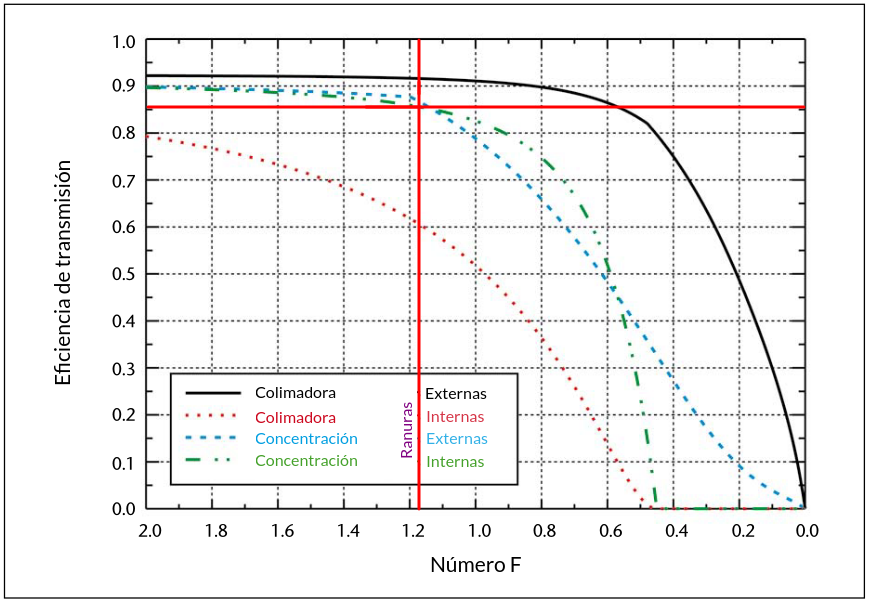
\includegraphics[
							width=\linewidth,
							height=85mm,
							keepaspectratio
						]{Desarrollo-experimental/Transmitancia.png}
						\caption{Valores de eficiencia idealizados de lentes de Fresnel calculadas en la reflexión de las superficies y otras pérdidas comunes.}
						\floatfoot{Imagen adaptada de \cite{davis_optical_2007}}
						\label{fig:Transmitancia}
					\end{figure}
					
					\begin{align}
						\gls{tau} &= \tau_{\text{lente}}\tau_{\text{cuarzo}} &= \percent{82.92}\label{equ:transmisión-cámara} \\
						\gls{tau} &= \tau_{\text{lente-ideal}}\tau_{\text{cuarzo}} &= \percent{92.56} \label{equ:transmisión-cámara-ideal}
					\end{align}
			
			\subsubsection{Radiación efectiva}
			
				La radiación que podría concentrar efectivamente esta lente de Fresnel sobre el recibidor solar se describe mediante~\eqref{equ:radiación-concentrada}; usando las asunciones generales propuestas se obtiene una radiación de \qty{51.80}{\watt}.
				
				\begin{equation}\label{equ:radiación-concentrada}
					\dot{Q}_{\text{absorbedor}} = \gls{intensity}_{\text{Sol}} \tau A_\text{Fresnel}
				\end{equation}
			
			
		
		\subsection{Diseño de la cámara de concentración solar}
			
			\subsubsection{Recibidor solar}
				
				Para el recibidor solar se comparó (\cref{table:comparacion-material-recibidor}) la propuesta de dos materiales típicamente usados para la manufactura de recibidores solares.
										
				\begin{longtblr}[
					caption = {Comparativa hallada entre los materiales propuestos para fungir como recibidor solar},
					label = {table:comparacion-material-recibidor},
				]{
					colspec = {l c *{2}{X[c]}},
					hlines,
					vlines,
					row{odd} = {bg=tablerowblue},
					row{1} = {
						bg = tabletitleblue,
						fg=white,
						font = \bfseries,
						halign=c
					},
					rowhead = 1,
					rows={m}
				}
					Propiedad & Unidades & Cobre & Carburo de Silicio\\
					Conductividad térmica 
						& \unit{\watt\per\m\kelvin}
						& \numrange{387.0}{430.0}% \cite{leonel_lira_cortes_conductividad_2010}
						& \numrange{120}{130}\\ % https://www.gab-neumann.com/Carburo-de-silicio-Propiedades https://geologiaweb.com/materiales/carburo-de-silicio/
					Coficiente de expansión térmica 
						& \unit{\per\degreeCelsius}
						& \num{16.5e-6}
						& \num{4e-6}\\
					Densidad
						& \unit{\kg\per\m\tothe{3}}
						& 8620
						& 3210\\
					Resistencia a la corrosión
						& ---
						& Menor
						& Mayor\\
					Costo
						& MXN
						& Menor
						& Mayor\\
					Accesibilidad
						& ---
						& Mayor
						& Menor\\
					Propiedades ópticas
						& ---
						& Alta reflectividad de luz en el espectro visible
						& Se puede manufacturar para tener buena absortividad
				\end{longtblr}
				
				A pesar de que el cobre tiene una alta reflectividad en el espectro de interés, se decide el uso de este material debido a sus ventajas de accesibilidad y costos. Para solventar el inconveniente descrito, se aplicó un recubrimiento que potencia sus características como recibidor solar usando el principio de selectividad espectral.
				
				Al inicio se consideró que el recubrimiento de óxido negro sería una opción adecuada ya que de acuerdo al resultado reportado en \cite{lowery_solar_1977}, alcanza valores de absortividad para el espectro solar en el rango de 0.78 a 0.86 y de emisividad de 0.04 a 0.08 convirtiéndose así en un candidato fuerte. 
				
				Este recubrimiento resulta favorable en términos de rendimiento, duración y preservación de propiedades del cobre; a pesar de ello, se decidió usar pintura de alta temperatura negra de uso industrial debido a varias ventajas halladas, entre ellas, la accesibilidad, costo y facilidad de uso sin mencionar que de acuerdo a \cite{mosquera_rivera_estudio_2020} donde se comparan diferentes pinturas para su aplicación en colectores solares, la  absortividad aplicada sobre cobre resulta de un \percent{95} superando al óxido negro.
								
				
				Se define entonces la temperatura máxima de forma ideal que podría alcanzar el concentrador solar considerando en función \cref{equ:areas-concentracion}.
				
				\begin{equation}
					\text{T}_{\text{recibidor}} = \dfrac{\alpha_{\text{Solar}} \gls{intensity}_{\text{Sol}}}{\epsilon_{\text{IR}} \gls{sigma-sb}} \times \gls{area-concentration-ratio}
				\end{equation}
				
				
				
	%			
	%			\begin{itemize}
	%				\item Se prepara una disolución de sales de ``ebolnol C'' en agua a una concentración de \qty{180}{\gram\per\litre}
	%				\item Se calienta la disolución a las instrucciones dadas por el fabricante o en su defecto a \qty{372}{\kelvin}.
	%				\item Se sumerge el área de interés sobre la 
	%			\end{itemize}
				
			\subsubsection{Almacenamiento térmico de calor}
				
				Como se ha resaltado a lo largo del texto, el sol es una fuente intermitente de energía, por lo que se propone un mecanismo de almacenamiento térmico de calor empleando arena de sílice de alta pureza la cual es una arena compuesta mayormente por \ch{SiO2}. Las propiedades más relevantes encontradas en \cite{davenport_thermal_2022} y \cite{wypych_2_2021} y por las que se decidió por este material se enumeran a continuación.
				
				\begin{itemize}
					\item \textbf{Excelente estabilidad térmica}: Se habla que la arena de sílice de cuarzo-$\alpha$ es estable hasta los \qty{573}{\degreeCelsius} donde sufre solamente una alteración de los ángulos en las uniones de la red cristalina para transformarse en cuarzo-$\beta$. Esta transformación es rápidamente reversible y no involucra ningún rompimiento de enlaces.
					\item \textbf{Alta capacidad calorífica}: En el estudio se observó que de temperatura ambiente hasta los \qty{1200}{\degreeCelsius} presenta una capacidad calorífica de \qtyrange{750}{1200}{\joule\per\kg\kelvin}
					\item \textbf{Conductividad térmica adecuada:} Gracias a que su conductividad no es demasiado alta ni demasiado baja (\qtyrange{7.2}{13.6}{\watt\per\m\kelvin}) no representa un problema hablando de pérdidas de calor.
					\item \textbf{Coeficiente de expansión térmica:} Posee un coeficiente de expansión térmica linear igual a \qty{14e-6}{\per\kelvin}.
					\item \textbf{Densidad}: \qty{2.65}{\g\per\cm\tothe{3}}
					\item \textbf{Humedad}: Aproximadamente \percent{0.1}
				\end{itemize}
				
			\subsubsection{Aislamiento térmico}
				
				Se realizó una investigación previa sobre los materiales candidatos como aislantes térmicos de los cuales se determinó que los siguientes materiales son potenciales candidatos: aereogel, fibra de sílice, fibra cerámica.
				
				\begin{longtblr}[
					caption = {Propiedades de los materiales aislantes térmicos},
					label = {table:comparacion-material-aislante},
				]{
					colspec = {X *{4}{c}},
					hlines,
					vlines,
					row{odd} = {bg=tablerowblue},
					row{1} = {
						bg = tabletitleblue,
						fg=white,
						font = \bfseries,
						halign=c
					},
					rowhead = 1,
					rows={m}
				}
					Parámetro & Unidades & Aereogel & Fibra de vidrio & Fibra cerámica\\
					Coeficiente de conductividad 
						& \unit{\watt\per\m\kelvin}
						& \numrange{0.02}{0.05}
						& \numrange{0.034}{0.044}
						& \numrange{0.06}{0.07}\\
					Rango de operación
						& \unit{\degreeCelsius}
						& \numrange{-200}{1000}
						& \numrange{-200}{700}
						& Hasta \num{1427}\\
					Ignífugo
						& ---
						& Sí
						& Sí
						& Sí\\
					Hidrófobo
						& ---
						& Sí
						& No
						& Sí	
				\end{longtblr}
				
				Como se observa, el aereogel y la fibra cerámica son excelentes candidatos, la decisión de usar aereogel fue tomada debido a su mínima densidad y a que es un material que se tiene disponible en el Departamento de Posgrado de Sistemas Dinámicos de la Unidad Profesional Interdisciplinaria en Ingeniería y Tecnologías Avanzadas.
			
			\subsubsection{General}
				
				En un inicio se contempló el uso de poliaftalamida para las paredes del desalinizador ya que es un termoplástico resistente a factores climáticos adversos durante largo tiempo e ideal para ser usado en exteriores además de tener baja absorción de humedad. En la~\cref{table:propiedades-poliaftalamida} se listan propiedades que se consideran importantes para el diseño.
				
				\begin{longtblr}[
					caption = {Propiedades de la poliaftalamida},
					label = {table:propiedades-poliaftalamida},
				]{
					colspec = {X[l] *{2}{X[c]}},
					hlines,
					vlines,
					row{odd} = {bg=tablerowblue},
					row{1} = {
						bg = tabletitleblue,
						fg=white,
						font = \bfseries,
						halign=c
					},
					rowhead = 1,
					rows={
						valign = m
					}
				}
					Parámetro & Unidad & Valor\\
					Densidad & \unit{\gram\per\cm\tothe{3}} & \numrange{1.2}{1.4}\\
					Temperatura de transición vítrea & \unit{\degreeCelsius} & \numrange{127}{140}\\
					Temperatura de fusión & \unit{\degreeCelsius} & \numrange{278}{285}
				\end{longtblr}
			
			A pesar de tener buenas cualidades para este diseño, se encontraron limitaciones en la disponibilidad y accesibilidad, por lo que se sustituyó con Nylamid M, el cual es un plástico ingenieril que posee propiedades de interés, tales como: buena resistencia mecánica, buena resistencia térmica, baja disipación de calor y la cualidad de ser de grado alimenticio.
							
		\subsection{Definición de la alimentación}
					
			\subsubsection{Definición del caudal}
			
				Se definirá el caudal suponiendo una transmisión perfecta y directa al agua usando el valor de $\dot{Q}_{\text{absorbedor}}$ en \eqref{equ:potencia-necesaria-sistema}.
				
				\begin{align*}
				\dot{m} &= \dfrac{\qty{51.80}{\watt}\times\alpha_{\text{recibidor}}}{\qty{2493.97}{\kilo\joule\per\kg}}
						& \dot{m} &= \dfrac{\qty{49.21}{\watt}}{\qty{2493.97}{\kilo\joule\per\kg}}
						& \dot{m} &= \qty{0.0197}{\gram\per\s}
				\end{align*}
				
				Se observa que el caudal (\qty{1.18}{\milli\litre\per\minute}) es bastante pequeño y sabiendo que la mayor parte del calor se iría en el cambio de fase, se considera que la ebullición no es el medio más adecuado para desalinizar el agua y se puede considerar que combinar los mecanismos de ebullición y evaporación tendrán un efecto sinérgico en la productividad del sistema.
				
				Entonces se redefine el flujo másico necesario como~\cref{equ:flujo-másico-redefinido} dando un caudal de \qty{9.12}{\milli\litre\per\minute}
				
				\begin{equation}\label{equ:flujo-másico-redefinido}
					\dot{m} = \dfrac{\qty{49.21}{\watt}}{\left[\qty{3.9895}{\kilo\joule\per\kg\kelvin} \left(\qty{94.7}{\degreeCelsius}-\qty{15.5}{\degreeCelsius}\right) \right]} = \qty{0.156}{\gram\per\s}
				\end{equation}
			
		\subsection{Materiales}
			
				\subsubsection{Componentes}
				
				Se consideró de acuerdo al caudal que el uso de una bomba peristáltica sería la opción adecuada ya que permiten trabajar con fluidos altamente agresivos al no tener contacto directo con el fluido además de proporcionar caudales generalmente bajos. En la~\cref{table:propiedades-bomba} se describe el modelo seleccionado tras una exhaustiva revisión de los modelos disponibles.
				
				
				
				\begin{longtblr}[
					caption = {Propiedades de la bomba peristáltica EZO-PMP},
					label = {table:propiedades-bomba},
				]{
					colspec = {X[l] *{2}{X[c]}},
					hlines,
					vlines,
					row{odd} = {bg=tablerowblue},
	%				row{1} = {
	%					bg = tabletitleblue,
	%					fg=white,
	%					font = \bfseries,
	%					halign=c
	%				},
					rowhead = 0,
					rows={
						valign = m
					},
					note{*} = {Después de la calibración (específicamente para la bomba adquirida). Veáse \cref{subsec:calibración}}
				}
					\SetCell[c=3]{bg = tabletitleblue, c}EZO-PMP &&\\
					Parámetro & Unidad & Valor\\
					Alimentación motor & \unit{\volt} & \numrange{12}{24}\\
					Alimentación controlador & \unit{\volt} & \numrange{3.3}{5}\\
					Caudal mínimo & \unit{\milli\litre\per\minute} & 0.5\\
					Caudal máximo & \unit{\milli\litre\per\minute} & 54\TblrNote{*}\\
					Precisión de flujo & \unit{\percent} & $\pm$ 1\\
					Altura de bombeo & \unit{\m} & 8.1\\
					Tamaño & \unit{\mm} & 37.5 x 48 x 112\\
					Precio aproximado & USD & 84.99\\
					Grado alimenticio & & Sí
				\end{longtblr}
								
				Para la extracción de vapor se considera adecuado el uso de mini ventiladores con protección IP. Los detalles del modelo propuesto se encuentran en la tabla~\cref{table:propiedades-extractor}.
				
				\begin{longtblr}[
					caption = {Propiedades del extractor},
					label = {table:propiedades-extractor},
				]{
					colspec = {X[l] *{2}{X[c]}},
					hlines,
					vlines,
					row{odd} = {bg=tablerowblue},
	%				row{1} = {
	%					bg = tabletitleblue,
	%					fg=white,
	%					font = \bfseries,
	%					halign=c
	%				},
					rowhead = 0,
					rows={
						valign = m
					}
				}
					\SetCell[c=3]{bg = tabletitleblue, c}UF3H3-500B &&\\
					Parámetro & Unidad & Valor\\
					Alimentación & \unit{\volt} & \numrange{2}{3.5}\\
					Potencia & \unit{\watt} & 0.29\\
					Temperatura de operación & \unit{\degreeCelsius} & \numrange{-10}{70}\\
					Caudal & \unit{\milli\litre\per\minute} & \num{16000}\\
					RPM & rpm & 17000\\
					Tamaño & \unit{\mm} & 17 x 17 x 3\\
					Masa & \unit{\gram} & 1.36\\
					Protección IP & --- & IP58 \\
					Precio aproximado & USD & 24.21
				\end{longtblr}
				
				Para la conexión entre las diferentes partes, se encontró que las magueras de polietileno son la opción más adecuada debido a sus propiedades de flexibilidad, rigidez, temperatura de funcionamiento y costo.
				
			\subsubsection{Sensores}
				
				Debido a la naturaleza altamente corrosiva de los fluidos con los que se está trabajando y pensando en la vida útil de los componentes así como en su ensable, se seleccionaron dos modelos de sensores de temperatura. 
				
				Para la parte que interactua directamente con el agua se seleccionó el termistor ``USP10981 Thermistor Probe'' ya que presenta dos ventajas: posee una carcasa de acero inoxidable y se puede montar mediante una rosca NPT de $\frac{1}{8}$''. Sin embargo, debido a su tamaño, costo y rango de temperatura, no resulta viable para monitorear la temperatura que alcanza el recibidor solar. Para ello se utilizó un termopar tipo K comercial con roscado de 6mm.